% Options for packages loaded elsewhere
\PassOptionsToPackage{unicode}{hyperref}
\PassOptionsToPackage{hyphens}{url}
%
\documentclass[
]{article}
\usepackage{amsmath,amssymb}
\usepackage{lmodern}
\usepackage{iftex}
\ifPDFTeX
  \usepackage[T1]{fontenc}
  \usepackage[utf8]{inputenc}
  \usepackage{textcomp} % provide euro and other symbols
\else % if luatex or xetex
  \usepackage{unicode-math}
  \defaultfontfeatures{Scale=MatchLowercase}
  \defaultfontfeatures[\rmfamily]{Ligatures=TeX,Scale=1}
\fi
% Use upquote if available, for straight quotes in verbatim environments
\IfFileExists{upquote.sty}{\usepackage{upquote}}{}
\IfFileExists{microtype.sty}{% use microtype if available
  \usepackage[]{microtype}
  \UseMicrotypeSet[protrusion]{basicmath} % disable protrusion for tt fonts
}{}
\makeatletter
\@ifundefined{KOMAClassName}{% if non-KOMA class
  \IfFileExists{parskip.sty}{%
    \usepackage{parskip}
  }{% else
    \setlength{\parindent}{0pt}
    \setlength{\parskip}{6pt plus 2pt minus 1pt}}
}{% if KOMA class
  \KOMAoptions{parskip=half}}
\makeatother
\usepackage{xcolor}
\usepackage[margin=1in]{geometry}
\usepackage{color}
\usepackage{fancyvrb}
\newcommand{\VerbBar}{|}
\newcommand{\VERB}{\Verb[commandchars=\\\{\}]}
\DefineVerbatimEnvironment{Highlighting}{Verbatim}{commandchars=\\\{\}}
% Add ',fontsize=\small' for more characters per line
\usepackage{framed}
\definecolor{shadecolor}{RGB}{248,248,248}
\newenvironment{Shaded}{\begin{snugshade}}{\end{snugshade}}
\newcommand{\AlertTok}[1]{\textcolor[rgb]{0.94,0.16,0.16}{#1}}
\newcommand{\AnnotationTok}[1]{\textcolor[rgb]{0.56,0.35,0.01}{\textbf{\textit{#1}}}}
\newcommand{\AttributeTok}[1]{\textcolor[rgb]{0.77,0.63,0.00}{#1}}
\newcommand{\BaseNTok}[1]{\textcolor[rgb]{0.00,0.00,0.81}{#1}}
\newcommand{\BuiltInTok}[1]{#1}
\newcommand{\CharTok}[1]{\textcolor[rgb]{0.31,0.60,0.02}{#1}}
\newcommand{\CommentTok}[1]{\textcolor[rgb]{0.56,0.35,0.01}{\textit{#1}}}
\newcommand{\CommentVarTok}[1]{\textcolor[rgb]{0.56,0.35,0.01}{\textbf{\textit{#1}}}}
\newcommand{\ConstantTok}[1]{\textcolor[rgb]{0.00,0.00,0.00}{#1}}
\newcommand{\ControlFlowTok}[1]{\textcolor[rgb]{0.13,0.29,0.53}{\textbf{#1}}}
\newcommand{\DataTypeTok}[1]{\textcolor[rgb]{0.13,0.29,0.53}{#1}}
\newcommand{\DecValTok}[1]{\textcolor[rgb]{0.00,0.00,0.81}{#1}}
\newcommand{\DocumentationTok}[1]{\textcolor[rgb]{0.56,0.35,0.01}{\textbf{\textit{#1}}}}
\newcommand{\ErrorTok}[1]{\textcolor[rgb]{0.64,0.00,0.00}{\textbf{#1}}}
\newcommand{\ExtensionTok}[1]{#1}
\newcommand{\FloatTok}[1]{\textcolor[rgb]{0.00,0.00,0.81}{#1}}
\newcommand{\FunctionTok}[1]{\textcolor[rgb]{0.00,0.00,0.00}{#1}}
\newcommand{\ImportTok}[1]{#1}
\newcommand{\InformationTok}[1]{\textcolor[rgb]{0.56,0.35,0.01}{\textbf{\textit{#1}}}}
\newcommand{\KeywordTok}[1]{\textcolor[rgb]{0.13,0.29,0.53}{\textbf{#1}}}
\newcommand{\NormalTok}[1]{#1}
\newcommand{\OperatorTok}[1]{\textcolor[rgb]{0.81,0.36,0.00}{\textbf{#1}}}
\newcommand{\OtherTok}[1]{\textcolor[rgb]{0.56,0.35,0.01}{#1}}
\newcommand{\PreprocessorTok}[1]{\textcolor[rgb]{0.56,0.35,0.01}{\textit{#1}}}
\newcommand{\RegionMarkerTok}[1]{#1}
\newcommand{\SpecialCharTok}[1]{\textcolor[rgb]{0.00,0.00,0.00}{#1}}
\newcommand{\SpecialStringTok}[1]{\textcolor[rgb]{0.31,0.60,0.02}{#1}}
\newcommand{\StringTok}[1]{\textcolor[rgb]{0.31,0.60,0.02}{#1}}
\newcommand{\VariableTok}[1]{\textcolor[rgb]{0.00,0.00,0.00}{#1}}
\newcommand{\VerbatimStringTok}[1]{\textcolor[rgb]{0.31,0.60,0.02}{#1}}
\newcommand{\WarningTok}[1]{\textcolor[rgb]{0.56,0.35,0.01}{\textbf{\textit{#1}}}}
\usepackage{graphicx}
\makeatletter
\def\maxwidth{\ifdim\Gin@nat@width>\linewidth\linewidth\else\Gin@nat@width\fi}
\def\maxheight{\ifdim\Gin@nat@height>\textheight\textheight\else\Gin@nat@height\fi}
\makeatother
% Scale images if necessary, so that they will not overflow the page
% margins by default, and it is still possible to overwrite the defaults
% using explicit options in \includegraphics[width, height, ...]{}
\setkeys{Gin}{width=\maxwidth,height=\maxheight,keepaspectratio}
% Set default figure placement to htbp
\makeatletter
\def\fps@figure{htbp}
\makeatother
\setlength{\emergencystretch}{3em} % prevent overfull lines
\providecommand{\tightlist}{%
  \setlength{\itemsep}{0pt}\setlength{\parskip}{0pt}}
\setcounter{secnumdepth}{5}
\ifLuaTeX
  \usepackage{selnolig}  % disable illegal ligatures
\fi
\IfFileExists{bookmark.sty}{\usepackage{bookmark}}{\usepackage{hyperref}}
\IfFileExists{xurl.sty}{\usepackage{xurl}}{} % add URL line breaks if available
\urlstyle{same} % disable monospaced font for URLs
\hypersetup{
  pdftitle={HUDM6122 Homework\_03},
  pdfauthor={Chenguang Pan},
  hidelinks,
  pdfcreator={LaTeX via pandoc}}

\title{HUDM6122 Homework\_03}
\author{Chenguang Pan}
\date{2023-02-19}

\begin{document}
\maketitle

\hypertarget{ex-3.1}{%
\subsection{Ex 3.1}\label{ex-3.1}}

\emph{Construct the scatterplot of the heptathlon data showing the
contours of the estimated bivariate density function on each panel. Is
this graphic more useful than the unenhanced scatterplot matrix?}

\textbf{MY SOLUTION:}

Here, I use the \texttt{MASS::kde2d()} function to estimate the
bivariate density of the data, and plot the contours of the density
using the \texttt{contour()} function.

\begin{Shaded}
\begin{Highlighting}[]
\SpecialCharTok{\textgreater{}} \CommentTok{\# import the package}
\ErrorTok{\textgreater{}} \FunctionTok{library}\NormalTok{(MVA)}
\SpecialCharTok{\textgreater{}} \FunctionTok{library}\NormalTok{(HSAUR2)}
\SpecialCharTok{\textgreater{}} \FunctionTok{data}\NormalTok{(heptathlon)}
\SpecialCharTok{\textgreater{}} \CommentTok{\# Create a scatterplot matrix with density contours}
\ErrorTok{\textgreater{}} \FunctionTok{pairs}\NormalTok{(heptathlon[, }\SpecialCharTok{{-}}\FunctionTok{ncol}\NormalTok{(heptathlon)], }\AttributeTok{upper.panel =} \ControlFlowTok{function}\NormalTok{(x, y) \{}
\SpecialCharTok{+}   \FunctionTok{points}\NormalTok{(x, y)}
\SpecialCharTok{+}\NormalTok{   den }\OtherTok{\textless{}{-}}\NormalTok{ MASS}\SpecialCharTok{::}\FunctionTok{kde2d}\NormalTok{(x, y)}
\SpecialCharTok{+}   \FunctionTok{contour}\NormalTok{(den, }\AttributeTok{add =} \ConstantTok{TRUE}\NormalTok{, }\AttributeTok{col =} \StringTok{"red"}\NormalTok{, }\AttributeTok{lwd =} \DecValTok{2}\NormalTok{)\})}
\end{Highlighting}
\end{Shaded}

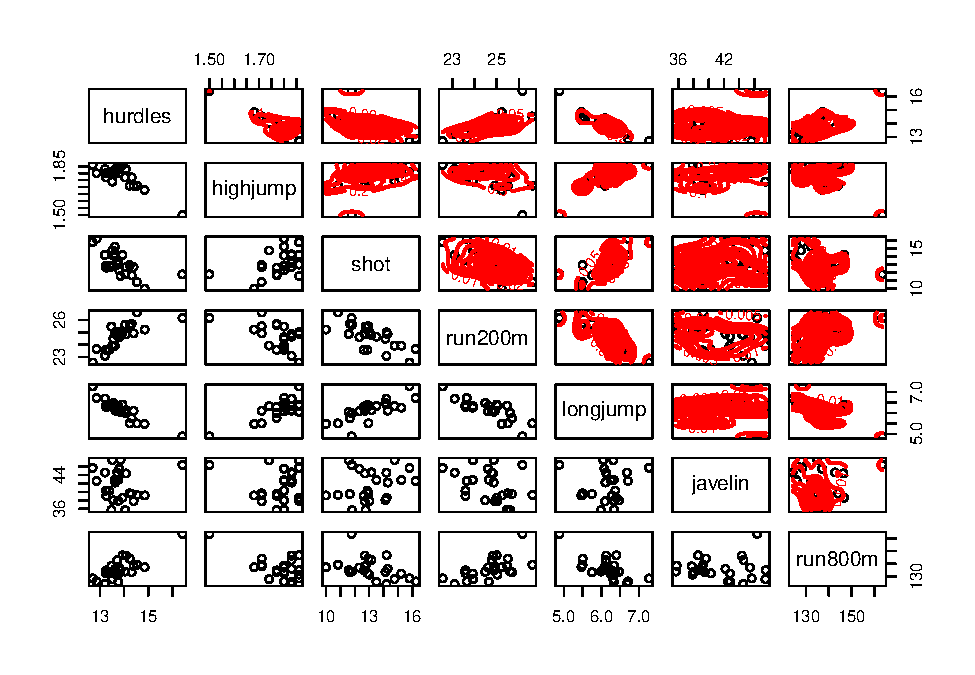
\includegraphics{HUDM6122-Homework_03-Chenguang-Pan_files/figure-latex/unnamed-chunk-1-1.pdf}

Comparing to the unenhanced scatter plot matrix, this mixed graph can
help to easily find the specific characteristics of joint distribution
of each pair, like the where is the center of the distribution.

\hypertarget{ex-3.2}{%
\subsection{Ex 3.2}\label{ex-3.2}}

\emph{Construct a diagram that shows the SO2 variable in the air
pollution data plotted against each of the six explanatory variables,
and in each of the scatterplots show the fitted linear regression and a
fitted locally weighted regression. Does this diagram help in deciding
on the most appropriate model for determining the variables most
predictive of sulphur dioxide levels?}

\textbf{MY SOLUTION:}

To solve this questions, I used the \texttt{ggplot2} to draw each graph
and use \texttt{gridExtra} to arrange the output's layout.

\begin{Shaded}
\begin{Highlighting}[]
\SpecialCharTok{\textgreater{}} \CommentTok{\# try to use a for{-}loop to get all the maps in fewer lines}
\ErrorTok{\textgreater{}} \FunctionTok{par}\NormalTok{(}\AttributeTok{mfrow=}\FunctionTok{c}\NormalTok{(}\DecValTok{2}\NormalTok{,}\DecValTok{3}\NormalTok{))}
\SpecialCharTok{\textgreater{}} \ControlFlowTok{for}\NormalTok{ (i }\ControlFlowTok{in} \FunctionTok{c}\NormalTok{(}\DecValTok{2}\SpecialCharTok{:}\DecValTok{7}\NormalTok{)) \{}
\SpecialCharTok{+}\NormalTok{   var\_name }\OtherTok{\textless{}{-}} \FunctionTok{paste0}\NormalTok{(}\StringTok{"p"}\NormalTok{,i}\DecValTok{{-}1}\NormalTok{)}
\SpecialCharTok{+}   
\SpecialCharTok{+}\NormalTok{   p }\OtherTok{\textless{}{-}} \FunctionTok{ggplot}\NormalTok{(USairpollution, }\FunctionTok{aes}\NormalTok{(}\AttributeTok{x =}\NormalTok{ USairpollution[,i], }\AttributeTok{y =}\NormalTok{ SO2)) }\SpecialCharTok{+} 
\SpecialCharTok{+}                 \FunctionTok{geom\_point}\NormalTok{() }\SpecialCharTok{+}
\SpecialCharTok{+}                 \FunctionTok{geom\_smooth}\NormalTok{(}\AttributeTok{method =} \StringTok{"lm"}\NormalTok{, }\AttributeTok{se =} \ConstantTok{FALSE}\NormalTok{, }\AttributeTok{color =} \StringTok{"blue"}\NormalTok{) }\SpecialCharTok{+}
\SpecialCharTok{+}                 \FunctionTok{geom\_smooth}\NormalTok{(}\AttributeTok{span =} \DecValTok{1}\NormalTok{, }\AttributeTok{se =} \ConstantTok{FALSE}\NormalTok{, }\AttributeTok{color =} \StringTok{"red"}\NormalTok{) }\SpecialCharTok{+}
\SpecialCharTok{+}                 \FunctionTok{labs}\NormalTok{(}\AttributeTok{title =} \FunctionTok{paste0}\NormalTok{(}\StringTok{"SO2 vs "}\NormalTok{, }\FunctionTok{colnames}\NormalTok{(USairpollution)[i]))}\SpecialCharTok{+}
\SpecialCharTok{+}                 \CommentTok{\# to remove the un{-}elegant x{-}axis name}
\SpecialCharTok{+}                 \FunctionTok{theme}\NormalTok{(}\AttributeTok{axis.title.x =} \FunctionTok{element\_blank}\NormalTok{(),}
\SpecialCharTok{+}                       \AttributeTok{axis.text.x =} \FunctionTok{element\_blank}\NormalTok{(),}
\SpecialCharTok{+}                       \AttributeTok{axis.ticks.x =} \FunctionTok{element\_blank}\NormalTok{())}
\SpecialCharTok{+}   \CommentTok{\# assign(var\_name, p)}
\SpecialCharTok{+}   \FunctionTok{print}\NormalTok{(p)}
\SpecialCharTok{+}\NormalTok{ \}}
\end{Highlighting}
\end{Shaded}

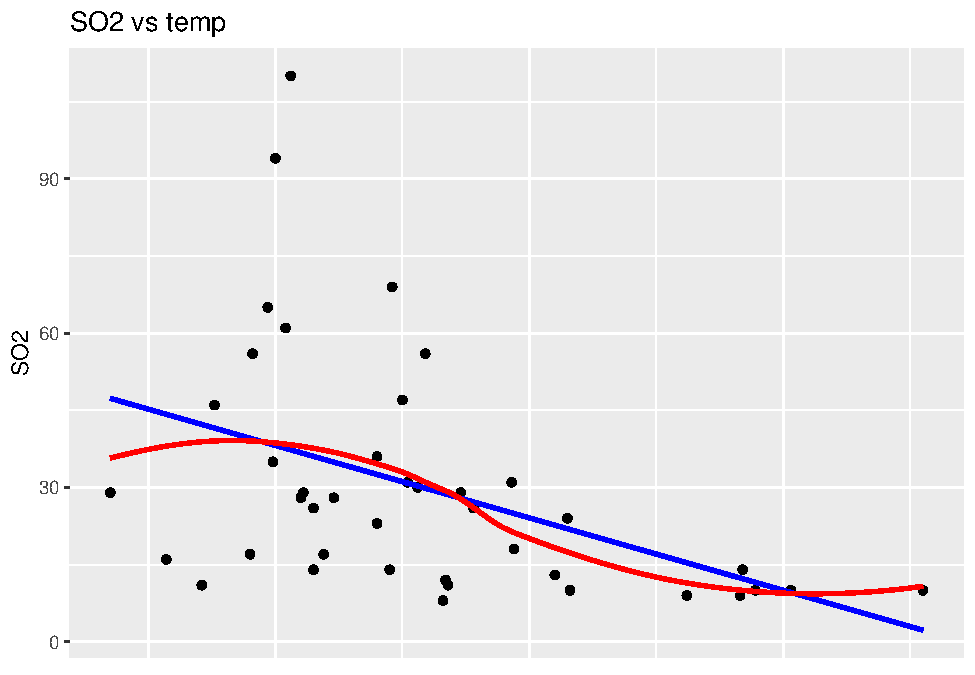
\includegraphics[width=0.5\linewidth,height=0.33\textheight]{HUDM6122-Homework_03-Chenguang-Pan_files/figure-latex/unnamed-chunk-3-1}
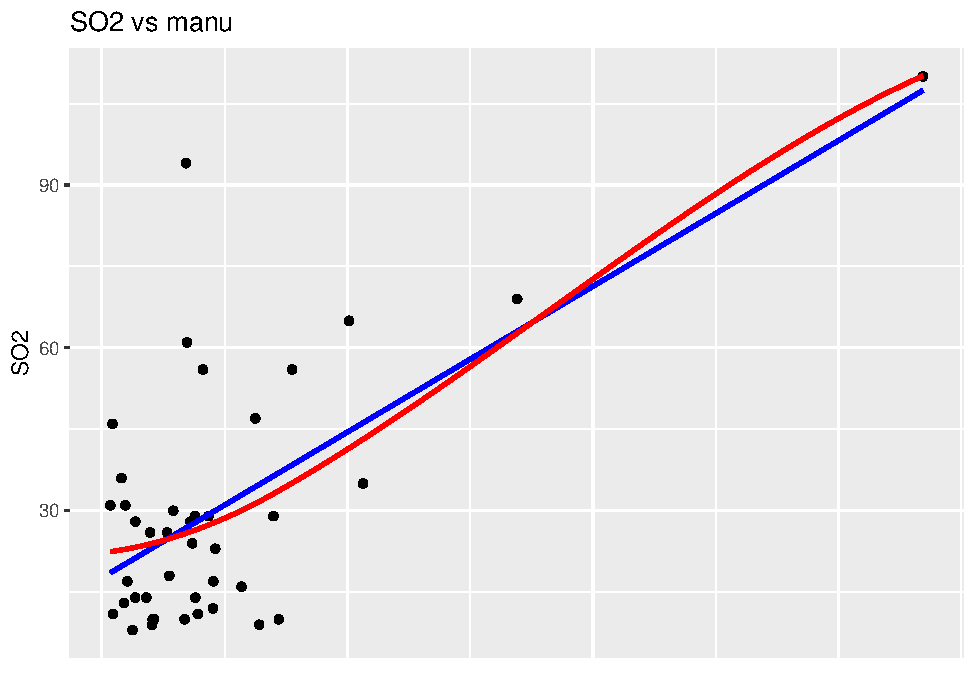
\includegraphics[width=0.5\linewidth,height=0.33\textheight]{HUDM6122-Homework_03-Chenguang-Pan_files/figure-latex/unnamed-chunk-3-2}
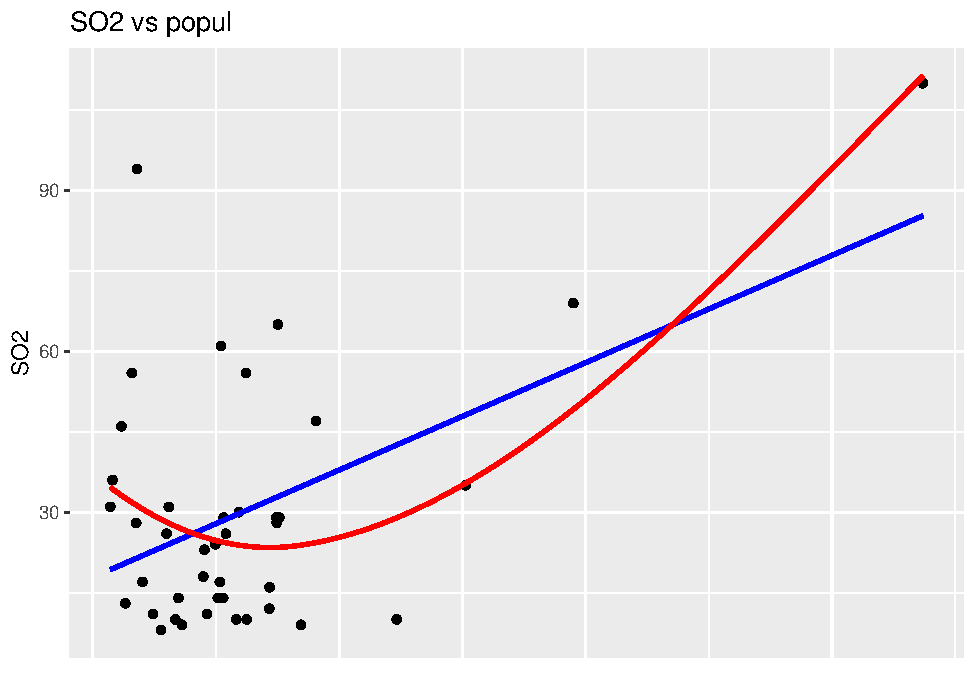
\includegraphics[width=0.5\linewidth,height=0.33\textheight]{HUDM6122-Homework_03-Chenguang-Pan_files/figure-latex/unnamed-chunk-3-3}
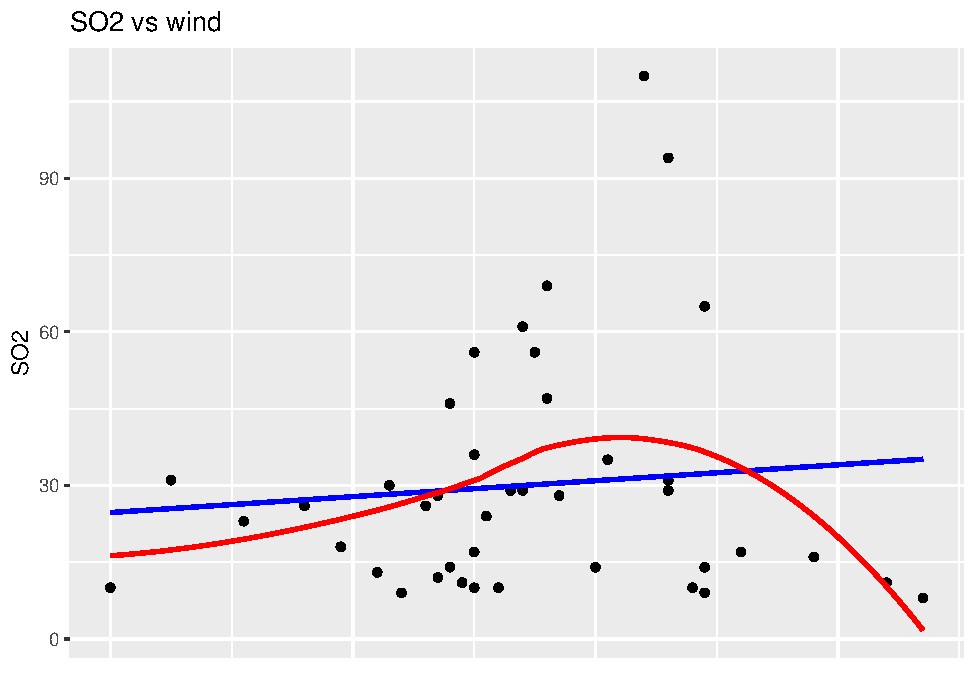
\includegraphics[width=0.5\linewidth,height=0.33\textheight]{HUDM6122-Homework_03-Chenguang-Pan_files/figure-latex/unnamed-chunk-3-4}
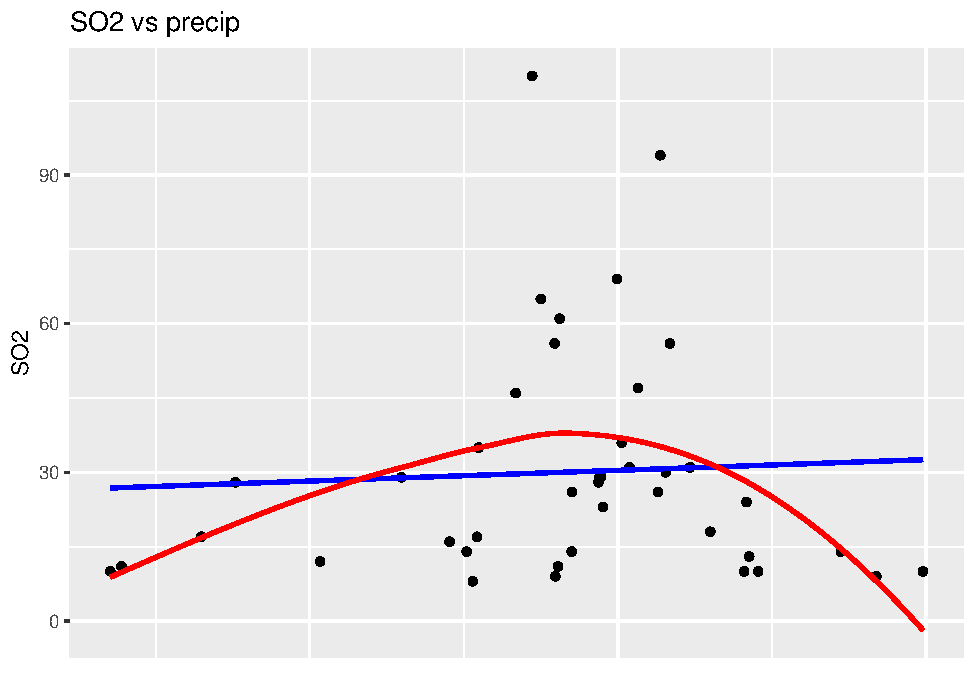
\includegraphics[width=0.5\linewidth,height=0.33\textheight]{HUDM6122-Homework_03-Chenguang-Pan_files/figure-latex/unnamed-chunk-3-5}
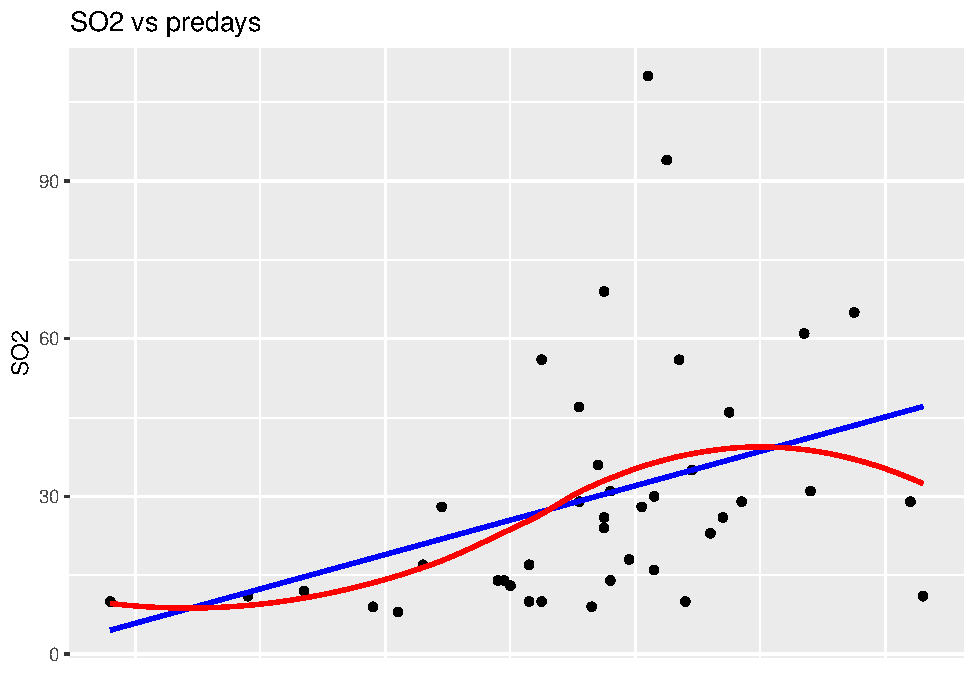
\includegraphics[width=0.5\linewidth,height=0.33\textheight]{HUDM6122-Homework_03-Chenguang-Pan_files/figure-latex/unnamed-chunk-3-6}
From six graphs above, we can not easily tell what the strongest
predictor is for predicting the \(SO_2\) concentration, since there are
some outliers with high leverage in each graph.

\end{document}
